In Aufgabe \ref{40000076} wurde die Grammatik
\begin{align*}
S&\to \varepsilon \\
S&\to SP \\
P&\to ZZ \\
Z&\to \texttt{a} \mid \texttt{b} \mid \texttt{c}
\end{align*}
für Wörter mit gerader Länge gefunden.
Bestimmen Sie den Parse Tree für die Ableitung der folgenden Wörter
\begin{teilaufgaben}
\item \texttt{abccba}
\item \texttt{ccccccaa}
\end{teilaufgaben}

\begin{loesung}
\begin{teilaufgaben}
\item
Durch Anwendung der Regel $S\to SP$ müssen erst genügend $P$ erzeugt werden,
aus denen dann die Terminalsymbole abgeleitet werden können:
\begin{center}
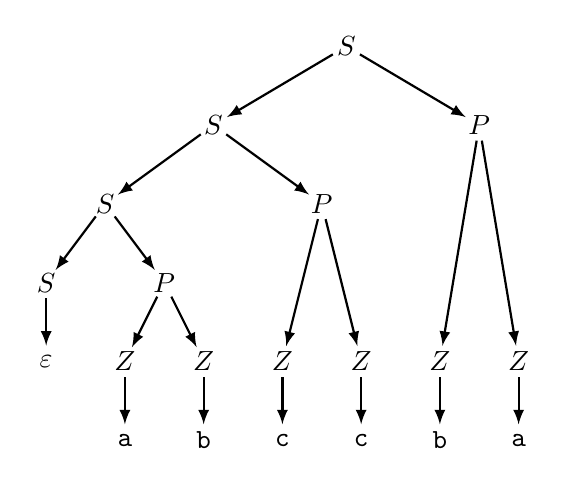
\begin{tikzpicture}[>=latex,thick]
\coordinate (S1) at (3.8125,0);
\coordinate (S2) at (2.125,-1);
\coordinate (S3) at (0.75,-2);
\coordinate (S4) at (0,-3);
\coordinate (P1) at (5.5,-1);
\coordinate (P2) at (3.5,-2);
\coordinate (P3) at (1.5,-3);
\coordinate (Z1) at (1,-4);
\coordinate (Z2) at (2,-4);
\coordinate (Z3) at (3,-4);
\coordinate (Z4) at (4,-4);
\coordinate (Z5) at (5,-4);
\coordinate (Z6) at (6,-4);
\coordinate (E) at (0,-4);
\coordinate (T1) at (1,-5);
\coordinate (T2) at (2,-5);
\coordinate (T3) at (3,-5);
\coordinate (T4) at (4,-5);
\coordinate (T5) at (5,-5);
\coordinate (T6) at (6,-5);
\node at (S1) {$S$};
\draw[->,shorten >= 0.2cm,shorten <= 0.2cm] (S1) -- (S2);
\draw[->,shorten >= 0.2cm,shorten <= 0.2cm] (S1) -- (P1);
\draw[->,shorten >= 0.2cm,shorten <= 0.2cm] (P1) -- (Z5);
\draw[->,shorten >= 0.2cm,shorten <= 0.2cm] (P1) -- (Z6);
\node at (S2) {$S$}; \node at (P1) {$P$};
\draw[->,shorten >= 0.2cm,shorten <= 0.2cm] (S2) -- (S3);
\draw[->,shorten >= 0.2cm,shorten <= 0.2cm] (S2) -- (P2);
\draw[->,shorten >= 0.2cm,shorten <= 0.2cm] (P2) -- (Z3);
\draw[->,shorten >= 0.2cm,shorten <= 0.2cm] (P2) -- (Z4);
\node at (S3) {$S$}; \node at (P2) {$P$};
\draw[->,shorten >= 0.2cm,shorten <= 0.2cm] (S3) -- (S4);
\draw[->,shorten >= 0.2cm,shorten <= 0.2cm] (S3) -- (P3);
\draw[->,shorten >= 0.2cm,shorten <= 0.2cm] (P3) -- (Z1);
\draw[->,shorten >= 0.2cm,shorten <= 0.2cm] (P3) -- (Z2);
\node at (S4) {$S$}; \node at (P3) {$P$};
\draw[->,shorten >= 0.2cm,shorten <= 0.2cm] (S4) -- (E);
\node at (E) {$\varepsilon$};
\node at (Z1) {$Z$};
\node at (Z2) {$Z$};
\node at (Z3) {$Z$};
\node at (Z4) {$Z$};
\node at (Z5) {$Z$};
\node at (Z6) {$Z$};
\draw[->,shorten >= 0.2cm,shorten <= 0.2cm] (Z1) -- (T1);
\draw[->,shorten >= 0.2cm,shorten <= 0.2cm] (Z2) -- (T2);
\draw[->,shorten >= 0.2cm,shorten <= 0.2cm] (Z3) -- (T3);
\draw[->,shorten >= 0.2cm,shorten <= 0.2cm] (Z4) -- (T4);
\draw[->,shorten >= 0.2cm,shorten <= 0.2cm] (Z5) -- (T5);
\draw[->,shorten >= 0.2cm,shorten <= 0.2cm] (Z6) -- (T6);
\node at (T1) {\texttt{a}};
\node at (T2) {\texttt{b}};
\node at (T3) {\texttt{c}};
\node at (T4) {\texttt{c}};
\node at (T5) {\texttt{b}};
\node at (T6) {\texttt{a}};
\end{tikzpicture}
\end{center}
\item
\begin{center}
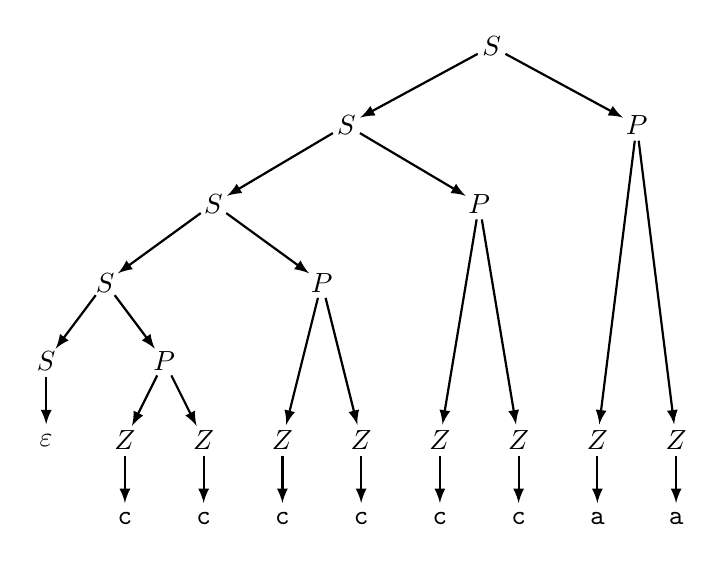
\begin{tikzpicture}[>=latex,thick]
\coordinate (S1) at (5.65625,0);
\coordinate (S2) at (3.8125,-1);
\coordinate (S3) at (2.125,-2);
\coordinate (S4) at (0.75,-3);
\coordinate (S5) at (0,-4);
\coordinate (P1) at (7.5,-1);
\coordinate (P2) at (5.5,-2);
\coordinate (P3) at (3.5,-3);
\coordinate (P4) at (1.5,-4);
\coordinate (Z1) at (1,-5);
\coordinate (Z2) at (2,-5);
\coordinate (Z3) at (3,-5);
\coordinate (Z4) at (4,-5);
\coordinate (Z5) at (5,-5);
\coordinate (Z6) at (6,-5);
\coordinate (Z7) at (7,-5);
\coordinate (Z8) at (8,-5);
\coordinate (E) at (0,-5);
\coordinate (T1) at (1,-6);
\coordinate (T2) at (2,-6);
\coordinate (T3) at (3,-6);
\coordinate (T4) at (4,-6);
\coordinate (T5) at (5,-6);
\coordinate (T6) at (6,-6);
\coordinate (T7) at (7,-6);
\coordinate (T8) at (8,-6);
\node at (S1) {$S$};
\draw[->,shorten >= 0.2cm,shorten <= 0.2cm] (S1) -- (S2);
\draw[->,shorten >= 0.2cm,shorten <= 0.2cm] (S1) -- (P1);
\draw[->,shorten >= 0.2cm,shorten <= 0.2cm] (P1) -- (Z7);
\draw[->,shorten >= 0.2cm,shorten <= 0.2cm] (P1) -- (Z8);
\node at (S2) {$S$}; \node at (P1) {$P$};
\draw[->,shorten >= 0.2cm,shorten <= 0.2cm] (S2) -- (S3);
\draw[->,shorten >= 0.2cm,shorten <= 0.2cm] (S2) -- (P2);
\draw[->,shorten >= 0.2cm,shorten <= 0.2cm] (P2) -- (Z5);
\draw[->,shorten >= 0.2cm,shorten <= 0.2cm] (P2) -- (Z6);
\node at (S3) {$S$}; \node at (P2) {$P$};
\draw[->,shorten >= 0.2cm,shorten <= 0.2cm] (S3) -- (S4);
\draw[->,shorten >= 0.2cm,shorten <= 0.2cm] (S3) -- (P3);
\draw[->,shorten >= 0.2cm,shorten <= 0.2cm] (P3) -- (Z3);
\draw[->,shorten >= 0.2cm,shorten <= 0.2cm] (P3) -- (Z4);
\node at (S4) {$S$}; \node at (P3) {$P$};
\draw[->,shorten >= 0.2cm,shorten <= 0.2cm] (S4) -- (S5);
\draw[->,shorten >= 0.2cm,shorten <= 0.2cm] (S4) -- (P4);
\draw[->,shorten >= 0.2cm,shorten <= 0.2cm] (P4) -- (Z1);
\draw[->,shorten >= 0.2cm,shorten <= 0.2cm] (P4) -- (Z2);
\node at (S5) {$S$}; \node at (P4) {$P$};
\draw[->,shorten >= 0.2cm,shorten <= 0.2cm] (S5) -- (E);
\node at (E) {$\varepsilon$};
\node at (Z1) {$Z$};
\node at (Z2) {$Z$};
\node at (Z3) {$Z$};
\node at (Z4) {$Z$};
\node at (Z5) {$Z$};
\node at (Z6) {$Z$};
\node at (Z7) {$Z$};
\node at (Z8) {$Z$};
\draw[->,shorten >= 0.2cm,shorten <= 0.2cm] (Z1) -- (T1);
\draw[->,shorten >= 0.2cm,shorten <= 0.2cm] (Z2) -- (T2);
\draw[->,shorten >= 0.2cm,shorten <= 0.2cm] (Z3) -- (T3);
\draw[->,shorten >= 0.2cm,shorten <= 0.2cm] (Z4) -- (T4);
\draw[->,shorten >= 0.2cm,shorten <= 0.2cm] (Z5) -- (T5);
\draw[->,shorten >= 0.2cm,shorten <= 0.2cm] (Z6) -- (T6);
\draw[->,shorten >= 0.2cm,shorten <= 0.2cm] (Z7) -- (T7);
\draw[->,shorten >= 0.2cm,shorten <= 0.2cm] (Z8) -- (T8);
\node at (T1) {\texttt{c}};
\node at (T2) {\texttt{c}};
\node at (T3) {\texttt{c}};
\node at (T4) {\texttt{c}};
\node at (T5) {\texttt{c}};
\node at (T6) {\texttt{c}};
\node at (T7) {\texttt{a}};
\node at (T8) {\texttt{a}};
\end{tikzpicture}
\end{center}
\end{teilaufgaben}
\end{loesung}
